\documentclass[11pt, a4paper]{paper}
\usepackage{amsmath}
\usepackage{graphicx}
\usepackage{subfig}

\title {\bf Jaal:: An Dual Tree Matching Approach to High Quality All-Quads Surface Meshing  } 
\author {
Chaman Singh Verma\thanks{csverma@cs.wisc.edu}, Tim Taugtes \thanks{tautges@mcs.anl.gov} }

\begin{document}
\maketitle
\abstract { 
Applications of All-Quad surface mesh are abound, but to the best of our knowledge, there does not
exist any reliable public domain All-Quads meshing implementation even for complex 2D domains. Among 
various techniques that have been proposed in the past, probably {\em triangle to quad} transformation is
the most intuitive, appealing, and most importantly, robust.

The main objective of the work is to relax convexity condition from Suneeta's tree matching algorithm
to produce an extremely fast and robust all -quad meshing algorithm. After generating topologically
an {\em All Quad Mesh} using matching algorithm, we improve the resulting mesh using simple clean-up operations,
and quadrilateral shape optimization libaries.

This All Quad Mesh algorithm is part of MOAB toolkit, which is an open source library supporting mesh infrastructure for 
petacscale field simulations.

We demonstrate the effectivness of our algorithm for both CAD and non-CAD geometrical models.
Initial experiments shows that our implementation is at least 100 times faster than the original
implementation of Suneeta's algorithm for generating topological correct mesh. Performance with
all the cleanup operations and optimization is also within some reasonable limits for some of the 
benchmarking models.
}

\section { Introduction }
Quadrilateral mesh generation have been used since late 70s by many commerical 
CFD codes. The importance of unstructured quadrilateral mesh for the complex 
geometries is well known, but it is extremely surprising to  know that 
(to the best of our knowledge) that there does not exist any open source 
All-Quads surface meshing algorithm at par with high visible unstructured 
triangular mesh i.e. {\em Triangle }. \cite{jonathan}

Quadrilateral mesh generation do not have the theoretically  
strong backup as the trinagle mesh generation, still we strongly believe that it is possible to engineering an All-Quad meshing algorithm with some 
set of heurtistics, known algorithms and optimization libraries that can 
produce an extremely high quality quadrilateral mesh for most of models of 
practical importance, if not all. 

In this work, we focus on {\em Triangle to Quad} transformation approach because 
of its simplicity and robustness. Our method is based on Suneeta's tree
matching algorithm, but we relax the convexity conditions in her algorithm and
instead of using {|em Q-Percolation Algorithm}, we use a slightly less
efficient {\em Percolation-Up } algorithm because we believe that mesh
generation and quality improvement must be two independent componenents in the
mesh generation toolkits. Once we have topologically acceptable quad mesh,
we apply simple {|em Quads CleanUp } operations and shape optimization library
{\em Mesquite} to improve the resulting mesh.

The rest of the paper is organized as follows: Section 1, describes Triangle to Quad tranformation using graph and tree matching algorithms. Section 2, descibes improving topologically correct but geometrically unacceptable quadrilateral mesh. Section 3 describes results for both CAD and non-CAD geometrical models.
Section 4. describes implementation details and finally in Section 5, we conclude this work.

% \begin{figure}
% \begin{center}
% \includegraphics[scale=0.4]{quadflow.eps}
% \caption{There are seven independent components in developing high quality all-quad meshing algorithm.}
% \end{center}
% \label{fig:flowchart}
%\end{figure} 
\section {Previous work on all-quad meshing algorithms}

\item {\em Maturity of  2D/3D triangle mesh generation}

\begin{itemize}
\item {\em Triangle to Quad-Transformation}
\item {\em Surface Parameterization }
\item {\em Spectral Quadrangulation }
\item {\em Quad-Dominated }
\item {\em Graph Matching }
\item {\em Circle Packing }
\end {itemize}

{\em Mesh Cleanup}

% Advancing front Recombination ( QMorph ) 
% ... ( Paving )
% Circle packing 
%Spectral Patches
% Global Parameterization
%Disk patches
% Graph Matching.
% Statement of Observations
%   Complexity and Functionality.
% Graph Matching 
%  Edmonds  
%  Suneeta
% Jaal: State its complexity.
%     Relaxation of Convexity
%     Bounded Quality.
% Implementation
%      Comp. Inden. of ( Tri, Global and 3D Alg.).
% Results
%      Fastest Known Implementation.
%      Robustness 2D/3D
% Conclusions
% Future Work.
%      Suneeta's Complexity estimation.

\section { Graph Matching Algorithm }

\begin{figure}
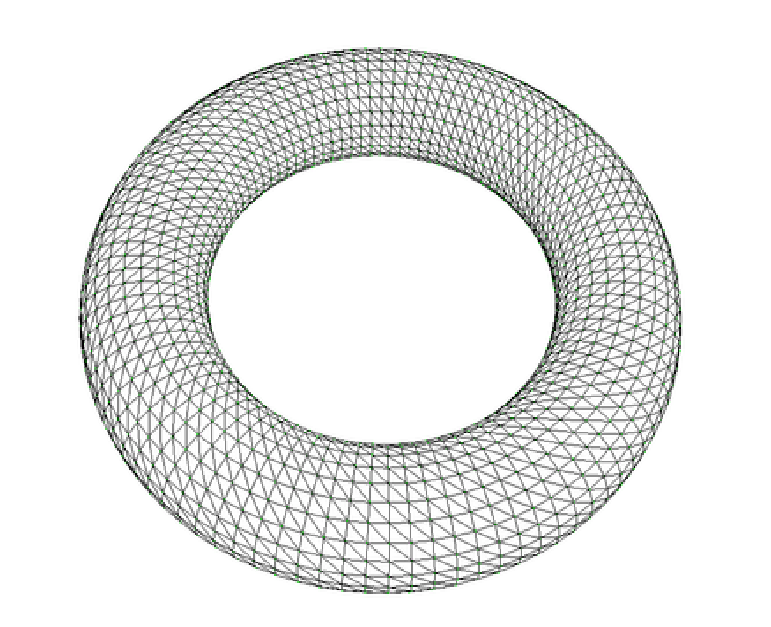
\includegraphics[scale=0.33]{torus1.eps}
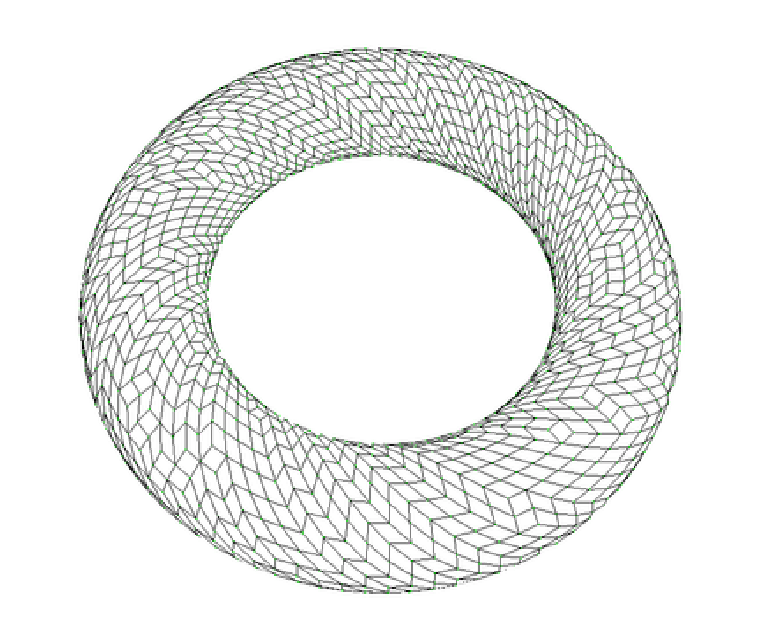
\includegraphics[scale=0.33]{torus2.eps}
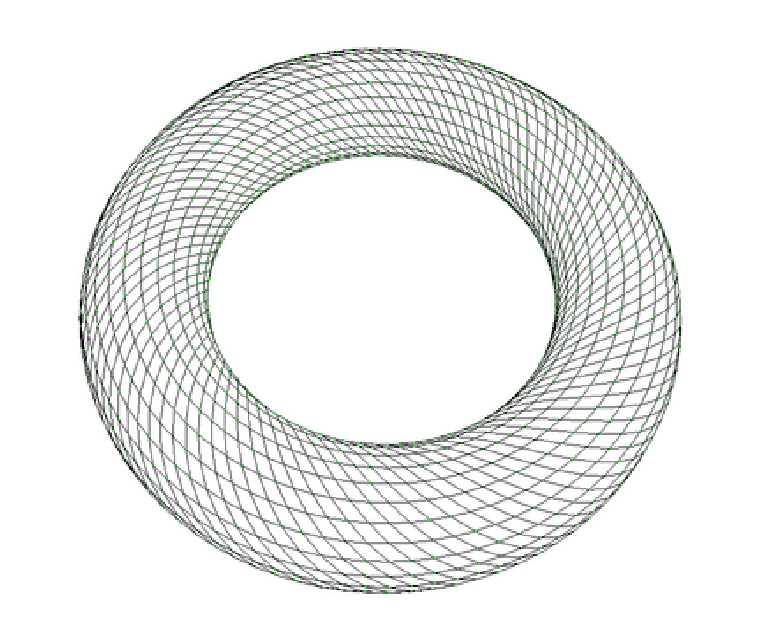
\includegraphics[scale=0.33]{torus3.eps}
\caption { (A) Input Triangle Mesh. (B) Quad Mesh using Edmonds Generalized
Graph Matching Algorithm (C) Quad Mesh using simplified Tree Matching Algorithm }
\end{figure}

%\begin{figure}
% \begin{center}
% \includegraphics[scale=0.5]{graphtree.eps}
% %\includegraphics[scale=0.4]{dfs.eps}
% %\includegraphics[scale=0.4]{bfs.eps}
% \caption{Converting Graph into a tree.}
% \end{center}
% \label{fig:graph_tree}
%\end{figure} 

\section { Topological Clean-up}
\subsection{ Quadrilateral Convexity }
\subsection{ Basic Operations}
\subsubsection{ Face Closing }
\subsubsection{ Face Opening }
\subsubsection{ Face Swapping }
\subsection { Advancing front clean-up}
\subsection { Boundary improvement}
\subsection { Volume Preserving Laplacian Smoothing}
\section {Results}
\section { Implementation details }

\section {Conclusions}
\end{document}
